% !TEX TS-program = XeLaTeX

% STYLE

\documentclass[a4paper, 12pt]{article}
\usepackage[left=1in,
		    right=1in,
    		    top=1in,
		    bottom=1in,
		    bindingoffset=0cm]{geometry}
		    \usepackage{array}
\usepackage{float}
\usepackage{graphicx}
\graphicspath{ {./images/} }
\usepackage{subfig}
\usepackage{enumerate}
\usepackage[normalem]{ulem} % underlining
\usepackage{booktabs} % tables
\usepackage[table]{xcolor} % coloring tables
\newcolumntype{L}[1]{>{\raggedright\let\newline\\\arraybackslash\hspace{0pt}}m{#1}} % beautiful column types
\newcolumntype{C}[1]{>{\centering\let\newline\\\arraybackslash\hspace{0pt}}m{#1}}

% LANGUAGE + FONT
		    
\usepackage[english]{babel}
\usepackage[backend=biber,
                     style=unified]{biblatex}
\newcommand{\citeay}[2][]{
   \citeauthor{#2} (\citeyear[#1]{#2})}
\addbibresource{ref.bib}
\usepackage{fontspec}  
\setmainfont{Minion 3}

% DRAWING

\usepackage{tikz}
\usepackage{tikz-qtree}
\usetikzlibrary{shapes.geometric}
\usetikzlibrary{trees,arrows}
\usetikzlibrary{positioning}
\usetikzlibrary{matrix}
\usetikzlibrary{tikzmark}
\usetikzlibrary{decorations.shapes}

% LINGUISTICS 

\usepackage{expex}
\usepackage[glossaries]{leipzig}
\makeglossaries
\newleipzig {npst} {npst} {non-past}
\newleipzig {nfin} {nfin} {non-finite}
\newleipzig {nsg} {nsg} {non-singular}

\lingset{numoffset=1ex, aboveexskip=1em, belowexskip=1em}

\title{Kazym Khanty schwa}
\author{Sasha Shikunova, EGG2023, Novi Sad}
\date{Last updated \today}

\begin{document}
\maketitle

	\section{Basic facts}
	
	Russia, Khanty-Mansi autonomous region, Kazym
	
	\begin{figure}[H]
		\centering
		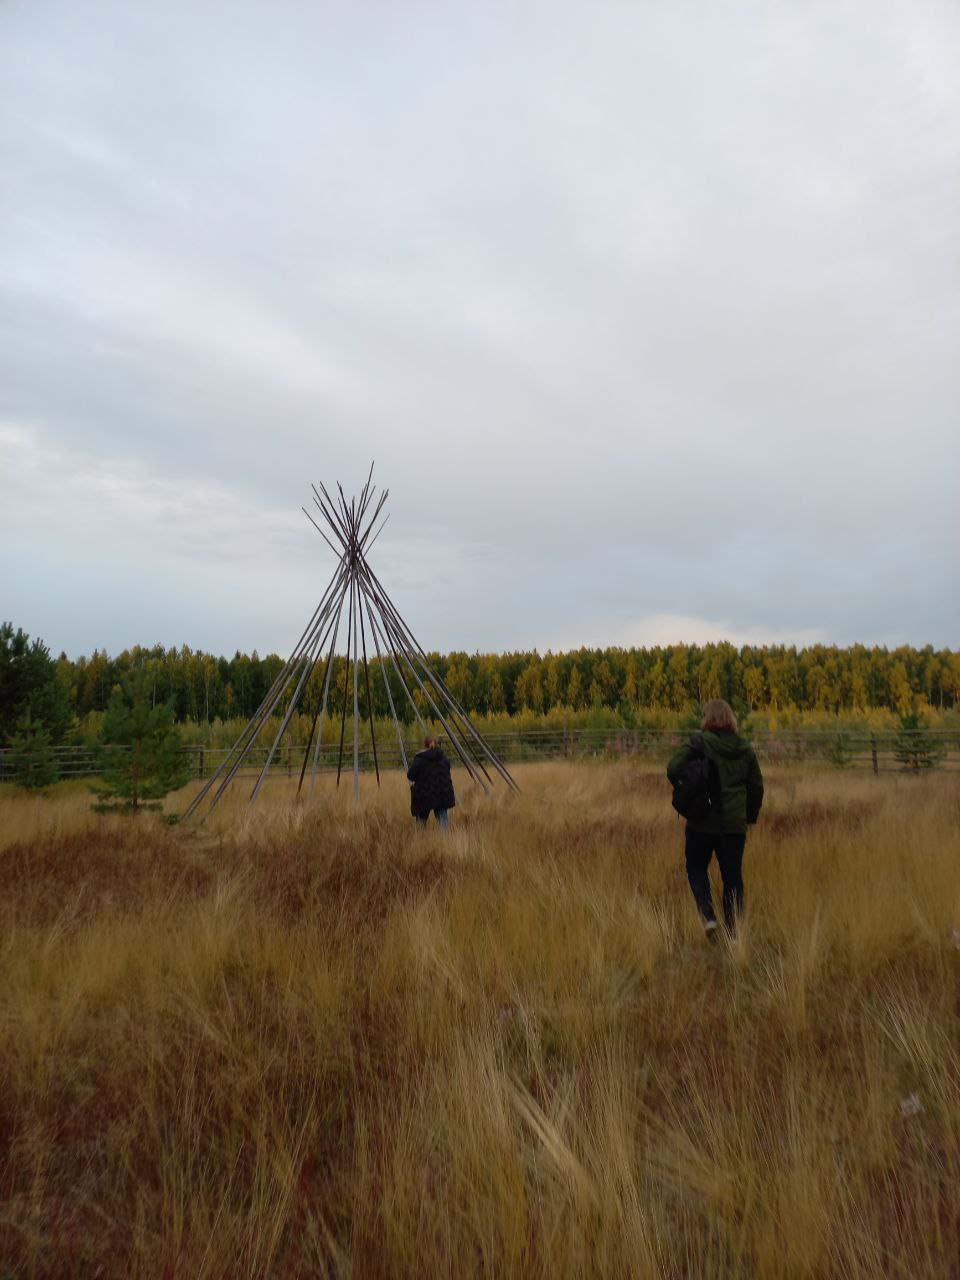
\includegraphics[scale=.167]{beginning}
		\hfill
		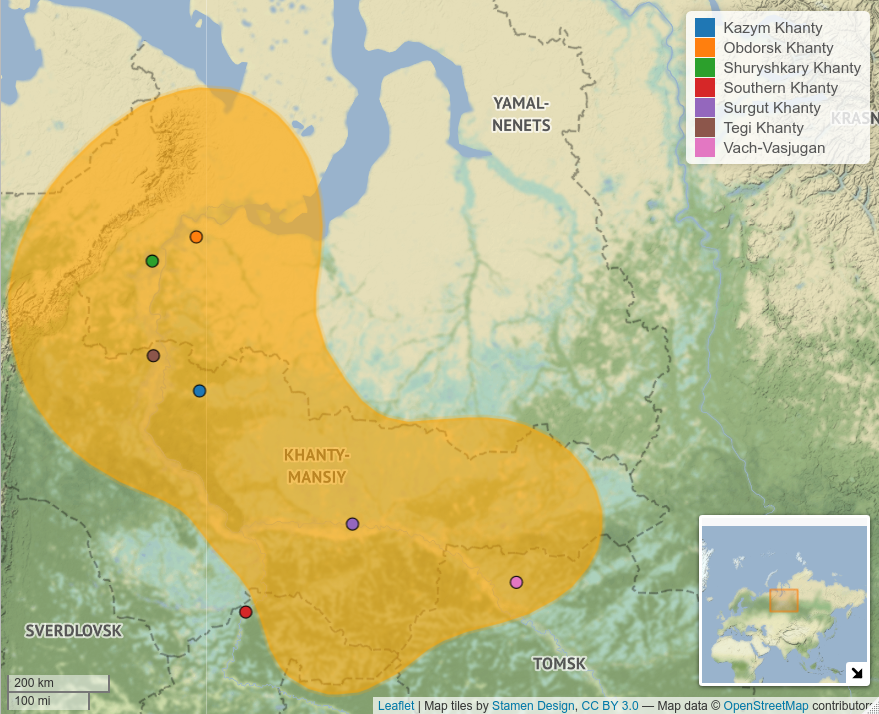
\includegraphics[scale=.4]{map}
	\end{figure}

	\noindent Vowel and consonant inventories \parencite{lketal2018}. In the practical transcription, λ = ɬ
	
	\begin{figure}[H]
		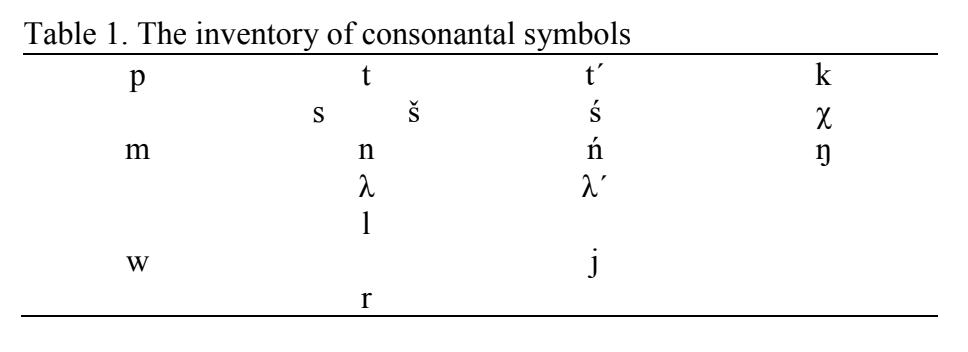
\includegraphics[scale=.66]{consonants}
	\end{figure}
	
	\newpage
	\noindent Not every vowel occurs in the first syllable:
	
	\begin{figure}[H]
		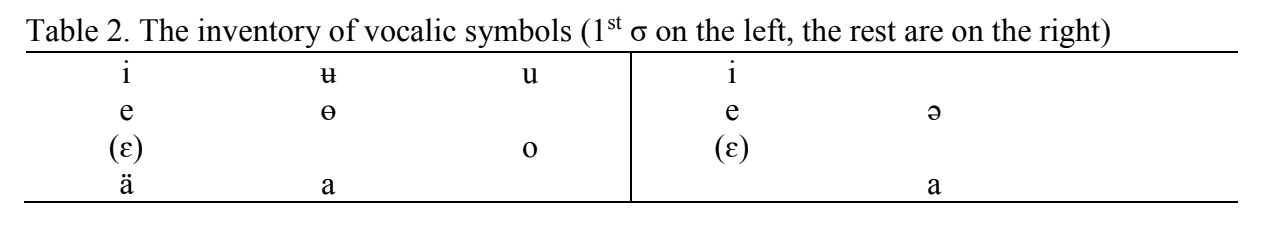
\includegraphics[scale=.66]{vowels}
	\end{figure}
	
\begin{enumerate}[$\gg$]
	\item No contrastive voicing
	\item Less vowel quality contrast in non-initial syllables (in native Khanty words; cf. \emph{kǎrtɵpka} `potato' -- Russian loanword)
\end{enumerate}
	Nominal inflection:

\begin{enumerate}[$\gg$]
	\item base - number - possessive - case (\ref{ex:nouninfl})
	
\ex
\begingl\label{ex:nouninfl}
	\gla jaj-λ-aλ-a//
	\glb brother-{\Pl}-{\Poss}.{\Tsg}-{\Dat}//
	\glft `{\Tsg}'s brother'//
\endgl
\xe
	
	\item if the base ends in /u i/, insertion of /w j/ is possible with some morphemes
	
	\pex 
		\a \emph{wʉλi} + \emph{(ə)n} $\rightarrow$ \emph{wʉλijn} `deer-{\Loc}'
		\a \emph{tɵ} + \emph{əm} $\rightarrow$ \emph{tʉw-əm} `carry-{\Nfin}.{\Pst}'
	\xe
	
\end{enumerate}
	Verbal inflection:

\begin{enumerate}[$\gg$]
	\item base - tense - inversive - agreement (\ref{ex:verbinfl})
	\item if the base ends in /u i/, insertion of /w j/ sometimes occurs (\emph{ari + (ə)s} $\rightarrow$ \emph{ari-js} `sing-{\Pst}')
	\item infinitive: base + \emph{ti/əm} ({\Npst}/{\Pst}); \emph{əm} after /u i/ causes insertion of /w j/ (\emph{tɵ-ti} `carry-{\Nfin}.{\Npst}' vs \emph{tʉw-əm} `carry-{\Nfin}.{\Pst}')
\end{enumerate}

\pex
\a\begingl\label{ex:verbinfl}
	\gla λɵt-s-aj-ən//
	\glb buy-{\Pst}-{\Pass}-{\Ssg}//
	\glft `you were bought'//
\endgl
\xe

	\section{Vowel-zero alternations}

	Schwa is a phoneme, see a minimal pair in (\ref{ex:minpair}). 
	
\pex\label{ex:minpair}
\a \emph{kurt} `iron'
\a \emph{kur-ət} `bull-{\Pl}'
\xe
	
	\noindent 3 types of verbal bases wrt. schwa behaviour:
	
\begin{table}[H]
\centering
\begin{tabular}{l c c c}
\toprule
\textbf{Form}
&
\textbf{No schwa}
&
\textbf{Alternating schwa}
&
\textbf{Stable schwa}
\\
\midrule
& 	ort- `divide' &		ir(ə)t- `turn' &		orət- `drag'\\
\addlinespace[0.2cm]
{\Npst}{[{\Tsg}]}& 	ort-əλ $\sim$ orλ &		irət-λ&		orət-λ\\
\addlinespace[0.2cm]
{\Pst}{[{\Tsg}]}&ort-əs&		irt-əs&orət-s		\\
\addlinespace[0.2cm]
{\Npst}-{\Ssg}&or-λ-ən&	irt-λ-ən	&	orət-λ-ən	\\
\addlinespace[0.2cm]
{\Pst}-{\Ssg}&or-s-ən&		irt-s-ən&	orət-s-ən	\\
\addlinespace[0.2cm]
{\Npst}-{\Fdu}&or-λ-əmn&	irt-λ-əmn	&	orət-λ-əmn	\\
\addlinespace[0.2cm]
{\Pst}-{\Fdu}&or-s-əmn&		irt-s-əmn&	orət-s-əmn	\\
\bottomrule
\end{tabular}
\label{t:verbpar}
\end{table}

	\noindent Vowel-final verb bases:

\ex Ca\#\\
\emph{χunta-s} `run-{\Pst}' --- \emph{χunta-s-n} `run-{\Pst}-{\Ssg}'
\xe

\ex Ci\#\\
\emph{arij-s} `sing-{\Pst}' --- \emph{ari-s-ən} `sing-{\Pst}-{\Ssg}'
\xe

\ex Cə\#\\
\emph{pɵrλə-s} `soar-{\Pst}' --- \emph{pɵrλə-s-n} `soar-{\Pst}-{\Ssg}'\\
also: \emph{pɵrλə-s-mən} `soar-{\Pst}-{\Fdu}'
\xe

	\pex[nopreamble=true] \label{ex:problem}
	\a {ari + əs} $\rightarrow$ {arijəs} $\rightarrow$ {arijs}
	\a {ari + əs + ən} $\rightarrow$ {ari + s + ən} \hfill \parencite{egorov2022}
	\xe
	
	\noindent Nominal inflection: possessive vs case markers
	
\begin{table}[H]
\centering
\begin{tabular}{l c c c}
\toprule
\textbf{Form}
&
\textbf{Ci\#}
&
\textbf{Ca\#}
&
\textbf{CVC\#}
\\
\midrule
& 	wʉλi `deer'&		λapka `shop'&		sʉmət (sʉmt) `birch'\\
\addlinespace[0.2cm]
{\Nom}& 	wʉλi&		λapka&		sʉmət (sʉmt)\\
\addlinespace[0.2cm]
{\Loc}&wʉλi-j(ə)n&		λapka-j(ə)n&sʉmət-n		\\
\addlinespace[0.2cm]
{\Poss}.{\Spl}&wʉλen&	λapka-j(ə)n	&	sʉmt-ən	\\
\bottomrule
\end{tabular}
\label{t:nompar}
\end{table}

	\section{Stress}
	
	Trochee with some quirks \parencite{tyutyunnikova2022}.
	
	\pex
	\a ˌpăsaˈnɛma \hfill păsan-ɛm-a `table-{\Poss}.{\Fsg}-{\Dat}'
	\a ˈλaraś \hfill λaraś `box'
	\a ˈλaraˈśɛma \hfill λaraś-ɛm-a `box-{\Poss}.{\Fsg}-{\Dat}'
	\a ˈλaraśa \hfill λaraś-a `box-{\Dat}'
	\a ˈpăsan \hfill păsan `table'
%	\a λaˈraś(ə)λa \hfill λaraś-(ə)λ-a `box-{\Poss}.{\Tsg}-{\Dat}'
	\a ˌmuχəˈλaja \hfill muχəλaja `around'
	\a ˌjuntˈλaλən \hfill junt-λ-aλ-ən `game-{\Pl}-{\Poss}.{\Tsg}-{\Loc}'
	\xe
	
	\noindent Interaction with schwa \parencite{tyutyunnikova2023}.
	
	\pex
	\a λaˈraśλa $\sim$ ˈλaraˈśəλa \hfill λaraś-(ə)λ-a `box-{\Poss}.{\Tsg}-{\Dat}'
	\a ˈpaknəλˈsəmn \hfill paknəλ-(ə)s-əm(ə)n `scare-{\Pst}-{\Tdu}'
	\a ˈpirśˈλaλən \hfill pir(ə)ś-λ-aλ-ən `old-{\Pl}-{\Poss}.{\Tsg}-{\Loc}'
	\a kɵrˈtəta $\sim$ ˈkɵrtəta \hfill kɵrt-ət-a `settlement-{\Pl}-{\Dat}'
	\a ˈsewrsaˈλəmn \hfill sew(ə)r-(ə)s-aλəm(ə)n `chop-{\Pst}-{\Fdu}>{\Nsg}'
	\xe
	
	\section{Summary of observations}

	Schwa is not always epenthetic:
	
\begin{enumerate}[$\gg$]
	\item There is a minimal pair where schwa makes the difference
	\item Schwa in the suffix can cause glide epenthesis -- sign of an underlying rather than an epenthetic vowel
\end{enumerate}
	Verbal bases can be divided into 3 classes:
	
\begin{enumerate}[$\gg$]
	\item Stable non-alternating schwa (\emph{orət-} `to drag')
	\item Alternating schwa (\emph{ir(ə)t-} `to turn')
	\item Consonant cluster never separated by schwa (\emph{ort-} `to divide')
\end{enumerate}
	In the verbal agreement suffix \emph{-əmən} `{\Fdu}' either of the two schwas can be present, depending on whether the base ends in a vowel or a consonant:
	
	\pex Schwa alternation in \emph{-əmən} `{\Fdu}'
		\a \emph{irt-s-əmn} `turn-{\Pst}-{\Fdu}' \hfill C\#
		\a \emph{orət-s-əmn} `drag-{\Pst}-{\Fdu}' \hfill C\#
		\a \emph{ji-s-mən} `become-{\Pst}-{\Fdu}' \hfill V\#
	\xe
	The schwa in the {\Ssg} suffix \emph{-ən} can disappear in the same circumstances as the initial schwa of \emph{-əmən} `{\Fdu}'.
	
	\pex Schwa alternation in \emph{-ən} `{\Ssg}'
		\a \emph{irt-s-ən} `turn-{\Pst}-{\Fdu}' \hfill C\#
		\a \emph{orət-s-ən} `drag-{\Pst}-{\Fdu}' \hfill C\#
		\a \emph{xunta-s-n} `run-{\Pst}-{\Fdu}' \hfill V\#
	\xe
	Alternating schwa seems to be lost after a full vowel but retained after another schwa; in contexts of vowel hiatus involving schwa, it is deleted:
	
	\pex Schwa alternation in \emph{-əmən} `{\Fdu}'; shown with supposed underlying schwas 
		\a \emph{irt-(ə)s-əm(ə)n} `turn-{\Pst}-{\Fdu}' \hfill C\#
		\a \emph{orət-(ə)s-əm(ə)n} `drag-{\Pst}-{\Fdu}' \hfill C\#
		\a \emph{ji-(ə)s-(ə)mən} `become-{\Pst}-{\Fdu}' \hfill V\#
	\xe
	There is occasional glide insertion after /i/-final bases, which is conditioned by the presence of overt agreement morphology after the tense marker:
	
\pex
	\a \emph{arij-s} `sing-{\Pst}' --- \emph{ari-s-ən} `sing-{\Pst}-{\Ssg}'
	\a \emph{arij-λ} `sing-{\Npst}' --- \emph{ari-λ-ən} `sing-{\Npst}-{\Ssg}'
\xe
	In the nominal paradigm, there is glide insertion before some suffixes (\ref{loc}) and vowel coalescence before others (\ref{poss}).
	
	\ex\label{loc}\emph{wʉλi} + \emph{ən} $\rightarrow$ \emph{wʉλij(ə)n} `deer-{\Loc}' \xe
	\ex~\label{poss}\emph{wʉλi} + \emph{ən} $\rightarrow$ \emph{wʉλen} `deer-{\Poss}.{\Spl}' \xe
	
	\section{Analysis}
	
	For the Khanty language, we need to account for the restrictions on clusters:
	
\begin{enumerate}[$\gg$]
	\item Word-initial clusters are prohibited $\Rightarrow$ Khanty has word-initial CV
	\item Word-final clusters are possible $\Rightarrow$ FENs can govern
\end{enumerate}
	There are three logically possible phonological representations of schwa:
	
\begin{enumerate}[$\gg$]
	\item Associated vowel: expected not to alternate with zero
	\item Floating vowel: expected to alternate with zero 
	\item Empty V-slot: expected to surface as zero except in a context that necessitates vowel epenthesis
\end{enumerate}
	I argue that all three logically possible schwas have to be recognised in Kazym Khanty.
	
		\subsection{Stable and alternating schwas}
		
	\begin{enumerate}[$\gg$]
		\item Stable schwa corresponds to an associated vowel that behaves similarly to full vowels in that it cannot alternate with zero:
		
		\pex Stable schwa in \emph{orət-} `drag'
			\a \emph{orət-s} \hfill `drag-{\Pst}'
			\a \emph{orət-s-ən} \hfill `drag-{\Pst}-{\Fdu}' 
		\xe
		
		\item Unstable, or alternating, schwa, the appearance of which is not explained by restrictions on clusters, corresponds to a floating vowel
		
		\pex The schwa in \emph{-ən} `{\Ssg}' can both occur and not occur inside a /sn/ cluster
			\a \emph{orət-s-ən} `drag-{\Pst}-{\Fdu}' \hfill C\#
			\a \emph{xunta-s-n} `run-{\Pst}-{\Fdu}' \hfill V\#
		\xe
		
		\item Epenthetic schwa in Khanty is expected to appear in illicit clusters
		\item Restrictions on clusters suggest that such contexts would include CCC\# or \#CC
		
			\pex Breaking up illicit clusters
		\a \emph{irətλ} /irtλ/ \hfill `turn.{\Npst}'
		\a \emph{əškola} /škola/ \hfill `school'
			\xe
		\item CCC\# $\rightarrow$ CəCC, \#CC $\rightarrow$ \#CəC
	\end{enumerate}
	What are the conditions under which an alternating/epenthetic schwa can be silenced?
	
	\begin{enumerate}[$\gg$]
		\item Alternating schwa occasionally appears in final closed syllables:
		
	\pex 
		\a \emph{kur-ət} \hfill `bull-{\Pl}'
		\a \emph{sʉmət} $\sim$ \emph{sʉmt} \hfill `birch'
	\xe
		
		\item Final CC clusters are still allowed:
		
	\pex
		\a \emph{kөrt} \hfill `settlement'
		\a \emph{λo{\'n}sʹ} \hfill `snow'
	\xe
		
		\item Hence, empty V-slot can be governed and silenced by FENs, whereas a floating schwa cannot (see \citeay{scheer2012yers} for a similar analysis of Polish yers)
	\end{enumerate}

		\subsection{Representation of \emph{-λ/-(ə)s}}
		
	How can we capture the difference between \emph{-λ/-(ə)s}?
	\begin{enumerate}[$\gg$]
		\item Non-past tense suffix \emph{-λ} never appears with a schwa before it:
			\pex
				\a \emph{irət-λ} \hfill `turn-{\Npst}'
				\a \emph{irt-λ-ən} \hfill `turn-{\Npst}-{\Ssg}'
				\a \emph{ari-jλ} \hfill `sing-{\Npst}'
			\xe
		\item Past tense suffix \emph{-(ə)s} is never preceded by schwa either, except for the final context after C\# bases:
			\pex
				\a \emph{irt-əs} \hfill `turn-{\Pst}'
				\a \emph{irt-s-ən} \hfill `turn-{\Pst}-{\Ssg}'
				\a \emph{ari-js} \hfill `sing-{\Pst}'
			\xe
		\item In non-word-final contexts, the behaviour of these suffixes is completely identical
		\item The representation of \emph{-λ} cannot contain schwa, whereas \emph{-(ə)s} can
		\item I propose the following representations:
		
\begin{minipage}[t]{.45\linewidth}
			\ex\label{fig:wulijn}\emph{-λ} `{\Npst}' \\
				\begin{tikzpicture}
\matrix [matrix of nodes, row sep=0.1em,
column sep={1.1em,between origins}]
{
|(c2)|{C} & |(v2)|{V}\\[0.4em]
|(C2)|{λ} & |(V2)|{}\\
};
\draw (c2.south) -- (C2.north);
				\end{tikzpicture}
			\xe
\end{minipage}	
\hfill
\begin{minipage}[t]{.45\linewidth}
			\ex\label{fig:wulijn}\emph{-(ə)s} `{\Pst}' \\
				\begin{tikzpicture}
\matrix [matrix of nodes, row sep=0.1em,
column sep={1.1em,between origins}]
{
|(r)|{ } & |(c2)|{C} & |(v2)|{V}\\[0.4em]
|(R)|{ə} & |(C2)|{s} & |(V2)|{}\\
};
\draw (c2.south) -- (C2.north);
				\end{tikzpicture}
			\xe
\end{minipage}	
	\item The floating schwa in the past tense \emph{-(ə)s} can associate to an empty V of the C\# base and govern the base-internal nucleus but after a V-final base, there is no empty slot
	\end{enumerate}
	There are two problems with having no schwa in \emph{-λ} `{\Npst}' and a floating schwa in \emph{-(ə)s} `{\Pst}':
	
	\begin{enumerate}[$\gg$]
		\item Identical behaviour in word-final context with V\# bases:
			\pex
				\a \emph{arij-s} `sing-{\Pst}' --- \emph{ari-s-ən} `sing-{\Pst}-{\Ssg}'
				\a \emph{arij-λ} `sing-{\Npst}' --- \emph{ari-λ-ən} `sing-{\Npst}-{\Ssg}'
			\xe
		\item There is a /rtλ/ cluster that is tolerated word-medially in \emph{irt-s-ən} `turn-{\Pst}-{\Fdu}'
	\end{enumerate}
	There has to be a contrast between the presence and absence of overt agreement morphology after \emph{-λ/-(ə)s}, since this is the condition on glide insertion:
	%	Nevertheless, the ability of associated schwa to govern makes correct predictions wrt. glide insertion, which is not possible in the presence of overt agreement morphology, i.e. when \emph{-λ/-(ə)s} are not word-final and the V before them is governed:

	
	\begin{enumerate}[$\gg$]
		\item Suppose /i/-final bases have a floating glide (there are lexical exceptions to the glide epenthesis rule)
			\pex Epenthesis is not automatic
				\a \emph{ari-js} \hfill `sing-{\Pst}'
				\a \emph{ji-s} \hfill `become-{\Pst}'
			\xe
		\item The schwa of the agreement marker governs the nucleus before \emph{-λ/-(ə)s}
		\item A governed slot cannot license the C for the glide should associate to
		\item No epenthesis results
		\item Still, there is a problem with \emph{-λ} `{\Npst}': the V before it can be governed by FENs
	\end{enumerate}
	
		\subsection{Schwas are controlled by the left context}
		
	Government and licensing operate from right to left. If only government and licensing were active in the Khanty schwa algorithm, we would not expect two different surface forms of \emph{-əmən} `{\Fdu}':

	\pex Schwa alternation in \emph{-əmən} `{\Fdu}'; shown with supposed underlying schwas 
		\a \emph{orət-(ə)s-əm(ə)n} `drag-{\Pst}-{\Fdu}' \hfill C\#
		\a \emph{xunta-(ə)s-(ə)mən} `run-{\Pst}-{\Fdu}' \hfill V\#
	\xe
	
	\begin{enumerate}[$\gg$]
		\item The left context makes the difference here: C\# bases are different from V\# bases
		\item This suggests that the mechanism of silencing alternating schwas is not government-based
		\item Alternating schwa can be incorporated and induce a stress shift:
		
		\pex
			\a \emph{ˈλa.raś} \hfill λaraś `box'
			\a \emph{λa.ˈraś.λa} $\sim$ \emph{ˈλa.ra.ˈśə.λa} \hfill λaraś-(ə)λ-a `box-{\Poss}.{\Tsg}-{\Dat}'
		\xe
		
		\item I suggest that schwas can be silenced when incorporated by a full (associated) vowel and subsequently deleted
		
	\pex Deriving \emph{mǎn-s-əmn} `go-{\Pst}-{\Fdu}'
		\a Underlying form: \emph{mǎn-(ə)s-(ə)m(ə)n}
		\a Associate what can be associated: \emph{mǎn-əs-əmən}
		\a Run projection and incorporation: \emph{mǎn-s-əmn}
	\xe
	
	\pex~Deriving \emph{xunta-s-mən} `run-{\Pst}-{\Fdu}'
		\a Underlying form: \emph{xunta-(ə)s-(ə)mən}
		\a Associate what can be associated: \emph{xunta-s-əmən}
		\a Run projection and incorporation: \emph{xunta-s-mən}
	\xe
		
		\item Schwas sometimes disappear after full vowels but always appear after another alternating schwa
		\item Underlyingly associated schwas are incorporating heads
		\item Floating schwas project to Line 1 and can be incorporated
		\item Empty nuclei do not project and are not incorporated, since Khanty stress is not weight-sensitive
	\end{enumerate}
	Can we still keep the analysis of glide insertion?
	
	\begin{enumerate}[$\gg$]
		\item Glide insertion is conditioned by the right context (overt agreement morphology)
		\item Vowel-zero in \emph{əmən} `{\Fdu}' is conditioned by the left context (final segment of the base)
		\item A compromise is an unsatisfactory system with complex rule ordering
	\end{enumerate}
	
	\pex Deriving \emph{ari-js} `sing-{\Pst}'
		\a Underlying form: \emph{ari(j)-(ə)s}
		\a Associate what can be associated (schwas only): \emph{ari(j)-əs}
		\a Run projection and incorporation: \emph{ari(j)-s}
		\a Associate glide if a licensed C is available: \emph{ari-js}
	\xe
	
	\pex~Deriving \emph{ari-s-ən} `sing-{\Pst}-{\Ssg}'
		\a Underlying form: \emph{ari(j)-(ə)s-(ə)n}
		\a Associate what can be associated (schwas only): \emph{ari(j)-əs-ən}
		\a Run projection and incorporation: \emph{ari(j)-s-ən}
		\a Associate glide if a licensed C is available: \emph{ari-s-ən}
	\xe
	
		\section{Nominal paradigm and morphosyntactic boundaries}
		
	In the nominal paradigm, there is a notable difference between possessive markers and case endings:
	
\begin{table}[H]
\centering
\begin{tabular}{l c c c}
\toprule
\textbf{Form}
&
\textbf{Ci\#}
&
\textbf{Ca\#}
&
\textbf{CVC\#}
\\
\midrule
& 	wʉλi `deer'&		λapka `shop'&		sʉmət (sʉmt) `birch'\\
\addlinespace[0.2cm]
{\Nom}& 	wʉλi&		λapka&		sʉmət (sʉmt)\\
\addlinespace[0.2cm]
{\Loc}&wʉλi-j(ə)n&		λapka-j(ə)n&sʉmət-n		\\
\addlinespace[0.2cm]
{\Poss}.{\Spl}&wʉλen&	λapka-j(ə)n	&	sʉmt-ən	\\
\bottomrule
\end{tabular}
\label{t:nompar}
\end{table}

	\begin{enumerate}[$\gg$]
		\item What is the difference between possessive \emph{(ə)n} and locative \emph{(ə)n}?
		\item I propose that there is a CV boundary between the base and the locative marker but none before the possessive
		\item The possessive is closer to the base in the functional sequence (\textsc{N < Num < Poss < K})
	\end{enumerate}
	
	\section*{Glossing abbreviations}
	
\printglossaries
	
\printbibliography

	\begin{figure}[H]
		\centering
		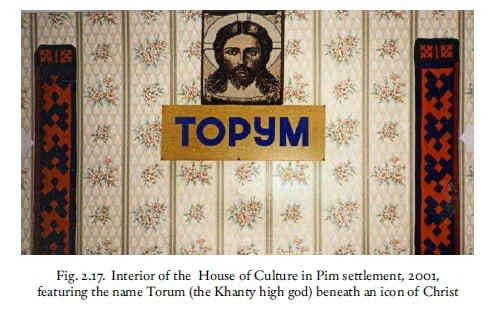
\includegraphics[scale=.66]{end}
	\end{figure}

\end{document}